%!TEX TS-program = xelatex
\documentclass[12pt, a4paper]{article}  

\usepackage{etex} % расширение классического tex в частности позволяет подгружать гораздо больше пакетов, чем мы и займёмся далее

%%%%%%%%%% Математика %%%%%%%%%%
\usepackage{amsmath,amsfonts,amssymb,amsthm,mathtools} 
%\mathtoolsset{showonlyrefs=true}  % Показывать номера только у тех формул, на которые есть \eqref{} в тексте.
%\usepackage{leqno} % Нумерация формул слева


%%%%%%%%%%%%%%%%%%%%%%%% Шрифты %%%%%%%%%%%%%%%%%%%%%%%%%%%%%%%%%
\usepackage{fontspec}         % пакет для подгрузки шрифтов
\setmainfont{Arial}   % задаёт основной шрифт документа

\defaultfontfeatures{Mapping=tex-text}

% why do we need \newfontfamily:
% http://tex.stackexchange.com/questions/91507/
\newfontfamily{\cyrillicfonttt}{Arial}
\newfontfamily{\cyrillicfont}{Arial}
\newfontfamily{\cyrillicfontsf}{Arial}

\usepackage{unicode-math}     % пакет для установки математического шрифта
\setmathfont{Asana Math}      % шрифт для математики
% \setmathfont[math-style=ISO]{Asana Math}
% Можно делать смену начертания с помощью разных стилей

% Конкретный символ из конкретного шрифта
% \setmathfont[range=\int]{Neo Euler}

\usepackage{polyglossia}      % Пакет, который позволяет подгружать русские буквы
\setdefaultlanguage{russian}  % Основной язык документа
\setotherlanguage{english}    % Второстепенный язык документа


%%%%%%%%%% Работа с картинками %%%%%%%%%
\usepackage{graphicx}                  % Для вставки рисунков
\usepackage{graphics}
\graphicspath{{images/}{pictures/}}    % можно указать папки с картинками
\usepackage{wrapfig}                   % Обтекание рисунков и таблиц текстом


%%%%%%%%%% Работа с таблицами %%%%%%%%%%
\usepackage{tabularx}            % новые типы колонок
\usepackage{tabulary}            % и ещё новые типы колонок
\usepackage{array}               % Дополнительная работа с таблицами
\usepackage{longtable}           % Длинные таблицы
\usepackage{multirow}            % Слияние строк в таблице
\usepackage{float}               % возможность позиционировать объекты в нужном месте
\usepackage{booktabs}            % таблицы как в книгах!
\renewcommand{\arraystretch}{1.3} % больше расстояние между строками

% Заповеди из документации к booktabs:
% 1. Будь проще! Глазам должно быть комфортно
% 2. Не используйте вертикальные линни
% 3. Не используйте двойные линии. Как правило, достаточно трёх горизонтальных линий
% 4. Единицы измерения - в шапку таблицы
% 5. Не сокращайте .1 вместо 0.1
% 6. Повторяющееся значение повторяйте, а не говорите "то же"
% 7. Есть сомнения? Выравнивай по левому краю!





%%%%%%%%%% Графика и рисование %%%%%%%%%%
\usepackage{tikz, pgfplots}  % язык для рисования графики из latex'a
\usepackage{amscd}                  %Пакеты для рисования
\usepackage[matrix,arrow,curve]{xy} %комунитативных диаграмм


%%%%%%%%%% Теоремы %%%%%%%%%%
\theoremstyle{plain}              % Это стиль по умолчанию.  Есть другие стили. 
\newtheorem{theorem}{Теорема}[section]
\newtheorem{result}{Следствие}[theorem]
% счётчик подчиняется теоремному, нумерация идёт по главам согласованно между собой

\theoremstyle{definition}         % убирает курсив и что-то еще наверное делает ;)
\newtheorem*{defin}{Определение}  % нумерация не идёт вообще

\newtheorem{fignia}{Какая-то фигня}




%%%%%%%%%% Свои команды %%%%%%%%%%
\usepackage{etoolbox}    % логические операторы для своих макросов


% Все свои команды лучше всего определять не по ходу текста, как это сделано в этом документе, а в преамбуле!


\usepackage{enumitem,pifont,xcolor}
\usepackage{fancyhdr}
 \DeclareMathOperator{\V}{Var}
\DeclareMathOperator{\cov}{Cov}
% Пакет, который ставит в каждом первом абзаце главы красную строку
% Просто, чтобы эта pdf-ка нормально смотрелась :)
\usepackage{indentfirst}
\setkeys{russian}{babelshorthands=true}


\title{Домашняя работа 3}
\date{\today}
\author{Перевышин Юрий}

\begin{document} % конец преамбулы, начало документа
	
	\maketitle
	
	\section{Упражнение. Свои команды}
	\subsection{Дисперсия и ковариация}
	$$\V(\varepsilon_i)=\sigma^2$$
	$$\cov(\varepsilon_i,\varepsilon_j)=0, \forall i\neq j$$
	\subsection{Сигма-алгебра}
	\newcommand{\s}{{\ensuremath{\sigma}}-~алгебра }
	Общеизвестный факт теории вероятности состоит в том, что  \s событий содержит достоверное событие.
	\subsection{Последовательности}
	\newcommand{\seqx}{{\ensuremath{x_1 \ldots x_n}} }
	\newcommand{\seqy}{{\ensuremath{y_1 \ldots y_n}}}
	Последовательность простых чисел \seqx является подпоследовательностью натуральных чисел \seqy.
	\subsection{Продвинутая последовательность}
	\newcommand{\seq}[2]{\ensuremath{x_{#1}\ldots x_{#2}}}
	Не очень понимаю практического значения этой команды, но у меня, таки, получилось её сделать
	демонстрирую: \seq{a}{z}, \seq{1}{6}, \seq{(a,b)}{(c,d)}
	\subsection{Синие точки}
	\begin{itemize} [label=\textcolor{blue}{\textbullet}] %работает с пакетом \usepackage{enumitem,pifont,xcolor}, подключен в преамбуле
		\item  Первый пункт 
		\item Второй пункт
		\item Третий пункт
	\end{itemize}
	
	%$\lim\limits_{x \to 0} \frac{\sin{x}}{x}$
	\subsection{Предел, как у взрослых}
	\newcommand{\llim}[2]{\ensuremath{\lim\limits_{#1}#2}} %чтобы воспользоваться командой нужно ввести два обязательных аргумента: 1. какая переменная, куда стремится, 2. выражение, от которого берется предел
	
	\llim{\gamma \to 1}{\frac{c^{1-\gamma}-1}{1-\gamma}} Кто возьмет, тому почет и уважуха!
	
	\subsection{Рисунки}
	
	\renewcommand{\thefigure}{\thesection:\arabic{figure}}
	
	\begin{figure} [h!]
		\begin{center}
			\caption{Национальная валюта}
			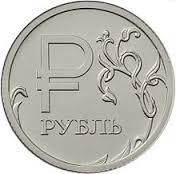
\includegraphics{Rubl1.jpg}
		\end{center}
	\end{figure}
	
	\subsection{Формулы}
	\renewcommand{\theequation}{Eq.(\arabic{equation})}
	
	\begin{equation} \label{eq:K_D}
	Y=K^\alpha L^{1-\alpha}
	\end{equation}
	
	
	\begin{equation}\label{eq:mrmc}
	MR=MC
	\end{equation}
	Формула \eqref{eq:K_D} называется функцией Кобба-Дугласа, а уравнение \eqref{eq:mrmc} задает условие максимизации прибыли фирмы-монополиста.
	\subsection{Переворачивающийся текст}
	Отсутствует
	
	\section{Задание 2}
	Чего-то даже идей нет никаких по этому поводу
	
	
\end{document} % конец документа

